\chapter{Studie an der DHBW Karlsruhe}
	Im folgenden Abschnitt werden die Durchführung der Studie sowie die genaueren Ergebnisse und Beobachtungen aufgeführt, welche im Verlauf der Studie gewonnen werden konnten. Es werden jedoch nur die reinen Beobachtungen und Ergebnisse hier aufgeführt, die Fazite werden erst in einem späteren Kapitel behandelt.
\section{Teilnehmerübersicht}
	Es folgt ein kurzer Überblick über die acht Teilnehmer der Studie.\\
	Insgesamt nahmen acht Kinder an den Terminen teil. Die Kinder waren zum Zeitpunkt dieser Arbeit noch in der Grundschule, jedoch nicht alle in der gleichen Klassenstufe. Die Kinder kannten sich zum Teil bereits untereinander bevor die Studie begann. Es wurde folgende Anzahl von Persönlichkeitstypen im Vorfeld abgegeben: drei Elefanten, zwei Border Collie, zwei Erdmännchen und ein Panda. Die Zuordnung der Tiere lautete wie folgt: Heinz, Lulu und Moritz als Elefanten, Jonas und Mario als Border Collies, Henriette und Benny als Erdmännchen und Sara als Panda.\\
	
	\begin{table}[H]
		\centering
		\begin{tabular}{|
				>{\columncolor[HTML]{C0C0C0}}c |c|c|c|}
			\hline
			\textbf{Typ} & \cellcolor[HTML]{C0C0C0}\textbf{Anzahl n} & \cellcolor[HTML]{C0C0C0}\textbf{Verteilung in \%} & \cellcolor[HTML]{C0C0C0}\textbf{Differenz in \%} \\ \hline
			ENTJ//INFJ   & 2                                         & 25                                                & +2,7                                             \\ \hline
			ENFJ//ESFJ   & 3                                         & 37,5                                              & -27,5                                            \\ \hline
			ISFP//INFP   & 2                                         & 25                                                & -16,4                                            \\ \hline
			INTJ//INFJ   & 1                                         & 12,5                                              & -5.7                                             \\ \hline
		\end{tabular}
		\begin{tabular}{|
				>{\columncolor[HTML]{C0C0C0}}c |c|c|c|}
			\hline
			\textbf{Typ} & \cellcolor[HTML]{C0C0C0}\textbf{Anzahl n} & \cellcolor[HTML]{C0C0C0}\textbf{Verteilung in \%} & \cellcolor[HTML]{C0C0C0}\textbf{Differenz in \%} \\ \hline
				E            & 5                                         & 62,5                                             & +1,0                                                 \\ \hline
				I            & 3                                         & 37,5                                             & -1,0                                                 \\ \hline
				T            & 3                                         & 33,3                                             & -28,5                                                \\ \hline
				F            & 6                                         & 66,6                                             & +28,5                                                \\ \hline
				S            & 5                                         & 62,5                                             & +4,6                                                 \\ \hline
				N            & 3                                         & 37,5                                             & -4,6                                                 \\ \hline
				J            & 6                                         & 75,0                                             & +23,8                                                \\ \hline
				P            & 2                                         & 25,0                                             & -23,8                                                \\ \hline
			\end{tabular}
		\caption[Verteilung der Typen unter den Teilnehmern]{Verteilung der Typen unter den Teilnehmern und Abweichung von Myers und Myers \cite[31]{myers_myers_2002}}
		\label{tab:distribution_type}
	\end{table}
	
	Die Tabelle \ref{tab:distribution_type} zeigt die Verteilung\footnote{Durch das Zusammenfassen von zweier Typen im Test kommen die Buchstaben T und F zusammen häufiger vor als es Teilnehmer gibt} der verschiedenen Persönlichkeitstypen in der oben genannten Gruppe der teilnehmenden Kinder. Dies sollte mit der Abbildung \ref{img:mbti_distribution} verglichen werden. Die Zahlen decken sich in manchen Fällen mit den Werten, welche von Myers-Briggs ermittelt wurden \cite[31]{myers_myers_2002}. Jedoch in den meisten Fällen liegen die Werte, die die Teilnehmer der Studie lieferten, deutlich neben den Werten von Myers-Briggs. Dies kann verschiedene Ursachen haben. Erstens, der Test ist auf Englisch, welches die Kenntnisse der Kinder übersteigt und deshalb die Eltern der Kinder helfen müssen und so unter Umständen verfälschte Werte herauskommen können. Zweitens, die Anzahl der Probanden, die diesen Test durchgeführt und die Werte übermittelt haben, liegen deutlich unter der Anzahl, die für Abbildung \ref{img:mbti_distribution} verwendet wurde. Daher ist eine größere Abweichung bei den Werten der Autoren dieser Arbeit nicht ungewöhnlich.
	
\section{Vorbereitung}
	Im folgenden Abschnitt wird der Beobachtungsbogen, welcher in Abbildung \ref{pdf:observation_sheets} dargestellt wird, genauer erläutert. Dieser Bogen wurde erstellt, bevor die Workshops begannen.\\
	Der Beobachtungsbogen besteht aus insgesamt drei Teilen. Der erste Teil soll das Verhalten der Kinder im Team dokumentieren. Als erstes Attribut wurde die Wichtigkeit des Teams beobachtet. Dabei wurde geschaut, wie sich das Kind im Team verhält, besonders ob es nicht die Einzelarbeit bevorzugt. Daher wurde auch beobachtet, ob das Kind in der Gruppe fähiger ist neue Themen zu lernen. Die Fähigkeit, generell in einem Team zu arbeiten, also ob es seinen Teampartnern hilft, sich querstellt oder eher der Einzelkämpfer ist. Um die Kommunikation zwischen den Teammitgliedern zu dokumentieren, wurde das Feedback der Kinder untersucht. Dabei wurde darauf geachtet, in wie weit Kinder sich gegenseitig, aber auch den Autoren gegenüber Feedback geben. Zusätzlich dazu wurde die generelle Kommunikation der Kinder untersucht. Um einen Rückschluss auf das Verhalten der Kinder in der Gruppe gegenüber Teammitgliedern schließen zu können, wurde beobachtet, ob Kinder versuchen, andere Kinder miteinzubeziehen in ihrer Arbeit als Gruppe und ob sie die Anmerkungen und Ideen anderer Kinder schätzen. Dazu wurde auch untersucht, ob sie jeden in der Gruppe als gleichwertiges Mitglied sehen. Gleichzeitig wurde auch beobachtet, wie gut die Kinder sich in einer Führungsrolle verhalten.
	
	Der zweite Beobachtungsblock bilden die kreativen Fähigkeiten, welche wiederum aufgeteilt sind in das divergierende\footnote{\gls{Divergenz}}, emergentes\footnote{\gls{Emergenz}} und konvergentes\footnote{\gls{Konvergenz}} Denken sowie die Einstellung gegenüber der Kreativität. Für den Block des divergierenden Denkens wurden vor allem die Ideen der Kinder beobachtet. Dabei spielten unter anderem das Ideenreichtum sowie die Originalität und die Flexibilität ihrer Ideen eine Rolle. Die Autoren schauten hierbei während Diskussionen über bestimmte Themen, ob die Kinder auch bei unbekannteren Themen Ideen hervorbringen. Vor allem sollte dadurch auch beobachtet werden, ob die Kinder in der Lage sind, aus anderen Perspektiven, im besten Fall sogar Perspektiven, welche ein Denken um mehrere Ecken erfordern, die Dinge zu betrachten und daraus Ideen zu generieren. Beim emergenten  Denken werden die Fähigkeiten der Abstraktion, detailgetreues Arbeiten und die Integrierfähigkeit untersucht. Für das detailgetreue Arbeiten wurde unter anderem untersucht, wie gut die Kinder in der Lage sind, Dinge zu visualisieren. Bei der Integration wurden die Kinder beobachtet, wie gut sie in der Lage sind, Verbindungen zwischen auf den ersten Blick nicht relevanten Dingen zu ziehen. Der Humor, die Fantasie, die emotionale Sensitivität sowie ihre Einstellung gegenüber Neuem wurden als Indikatoren dafür verwendet, wie die Haltung der Kinder zur Kreativität ist. Als letzter Block der kreativen Fähigkeiten wurde das generelle logische Denken der Kinder beobachtet.Der gesamte Kreativitäts-Block basiert auf dem Torrance Test (vgl. Kapitel \ref{sec:torrance_tests}).
	
	Die beiden eben beschriebenen Blöcke werden durch subjektive Beschreibungen der Autoren ausgefüllt, während der dritte und letzte Block, die Computational Thinking Skills, nur mit den vier Kategorien not able (ist nicht in der Lage), understands when shown (versteht es, nachdem es erklärt wurde), on their own (versteht es von selbst) und adding own ideas to it (ergänzt durch eigene Ideen) bewertet wird. Dabei wurde eine Werteskala von 0 bis 3 definiert, wobei den eben genannten Kategorien in der Reihenfolge jeweils eine Zahl zugeordnet ist. Zusätzlich dazu gibt es für den Fall, dass dieser Aspekt nicht beurteilt werden kann, die Kategorie  n/a (nicht angegeben). Die Computational Thinking Skills können in fünf Blöcke kategorisiert werden: Dekompositon, Generalisierung, algorithmisches Denken, Evaluation und Abstraktion. Dekomposition bewertet die Kinder auf ihre Fähigkeit ein Problem zu beschreiben und zu zerlegen sowie Lösungskriterien zu definieren. Die Generalisierung soll zeigen, wie gut die Kinder in der Lage sind, Muster und Konzepte, welche bereits gelernt wurden, wiederzuverwenden. Inwiefern die Kinder algorithmische Konzepte kennen und Schritte, welche zu einem Ergebnis führen definieren und implementieren können, wird durch das algorithmische Denken bewertet. Der Block Evaluation soll dokumentieren, ob am Ende das Programm der Kinder funktioniert, eventuelle Fehler gelöst werden konnten, warum ihr Programm das vorausgegangene Problem löst und ob die Kinder in der Lage sind, alternative Lösungsansätze zu finden. Zu guter Letzt wird durch die fünf Kategorien das Abstraktionsverhalten bewertet. Dieses setzt sich zusammen aus der Fähigkeit, das wichtigste Teil einer Lösung herauszuarbeiten, das wichtigste Detail zu nennen sowie eine Verbindung zwischen der Lösung und dem Erfolgskriterium zu schaffen.
 
\section{Durchführung}
	Vor Beginn der Studie führten alle Teilnehmer einen Persönlichkeitstest durch, der jedes der teilnehmenden Kinder einem Tier zuordnete. Der Test besteht aus 38 verschiedenen Fragen, jede dieser Frage bietet zwei Antwortmöglichkeiten. Am Ende dieses Tests bekommt der Teilnehmer als Ergebnis ein Tier entweder aus der Kategorie der extrovertierten oder der introvertierten Persönlichkeitstypen (vgl. Abbildung \ref{img:animals}). 
	\begin{figure}[htbp!]
		\centering
		\fbox{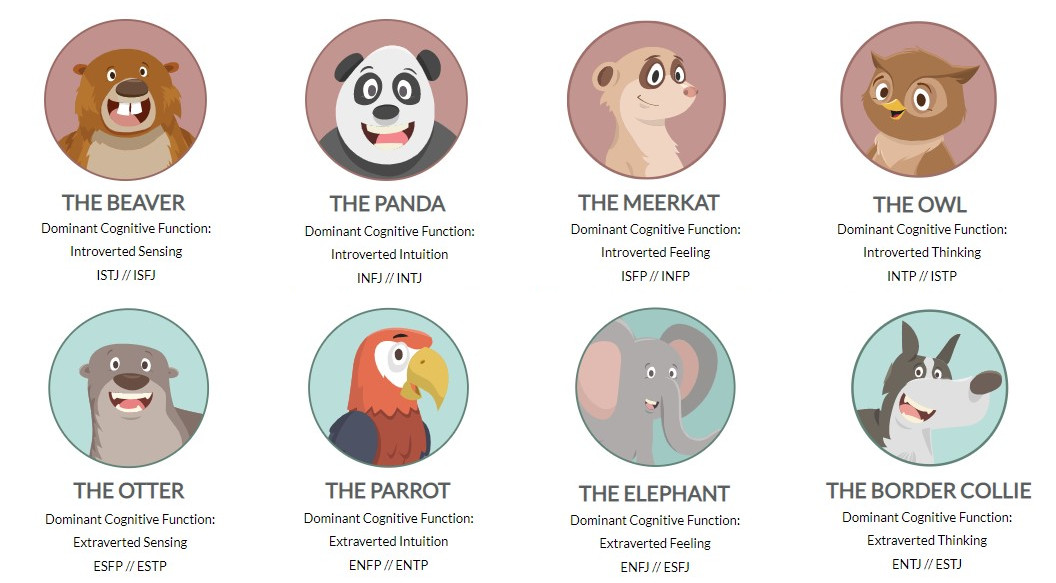
\includegraphics[width=0.4\textheight,angle=0]{img/animals}}
		\caption[Alle Tiere des Persönlichkeitstests]{Alle Tiere des Persönlichkeitstests \cite{knowAndLove}}
		\label{img:animals}
	\end{figure} 
	In der ersten Stunde der Studie mussten alle Teilnehmer den Computational Thinking Test durchführen. Die Auswertung der Ergebnisse aus der ersten Stunde jedes Teilnehmers befinden sich in Tabelle \ref{tab:data}. Wie bereits erwähnt, besteht dieser Test aus mehreren Kategorien, die normalisierten Ergebnisse befinden sich in Abbildung \ref{img:auswertung}.\\
	Die Termine der Studie können in zwei Phasen eingeteilt werden. Die erste Phase ist die Phase, in der die Kinder sich mit Lego WeDo vertraut machten. Die jeweiligen Termine hatten ein eigenes Thema, welches von der WeDo-App angeboten wurde. Die Autoren stellten zu Beginn eines Termins den Kindern Fragen zum Thema und es wurde über das Thema diskutiert. Nachdem die Diskussionsrunde vorbei war, führten die Kinder selbständig die von der WeDo-App bereitgestellten Kurse zu dem Thema durch während die Autoren die Kinder beobachteten und dabei Notizen in einem Fragebogen machten. Der Fragebogen wird im weiteren Verlauf noch genauer erklärt. Die zweite Phase läutete den Beginn des Wettbewerbs ein. Die beiden Gruppen, je vier Teilnehmer, erhielten ein sogenanntes Motivationsset von Lego, welches zusätzlich zu den bis dahin verwendeten Kästen verwendet wurden. Der Aufbau dieser Termine ähnelte dem von Phase eins: Jeder Teilnehmer bekam mit dem Motivationsset ein sogenanntes IngenieurInnen-Notizbuch (vgl. Abbildung \ref{img:explorer_heft}). In jedem Heft sind Aufgaben für die Kinder, insgesamt existieren 12 dieser Treffen, welche alle auf den Wettbewerb hinführen. Bei jedem dieser Treffen wird ein Thema, wie bereits in Phase eins besprochen, bevor die Kinder anschließend selbständig die weiteren Aufgaben lösten. Auch hier notierten die Autoren das Verhalten der Kinder und trugen dies in den Fragebogen ein. 
	\begin{figure}[htbp!]
		\centering
		\fbox{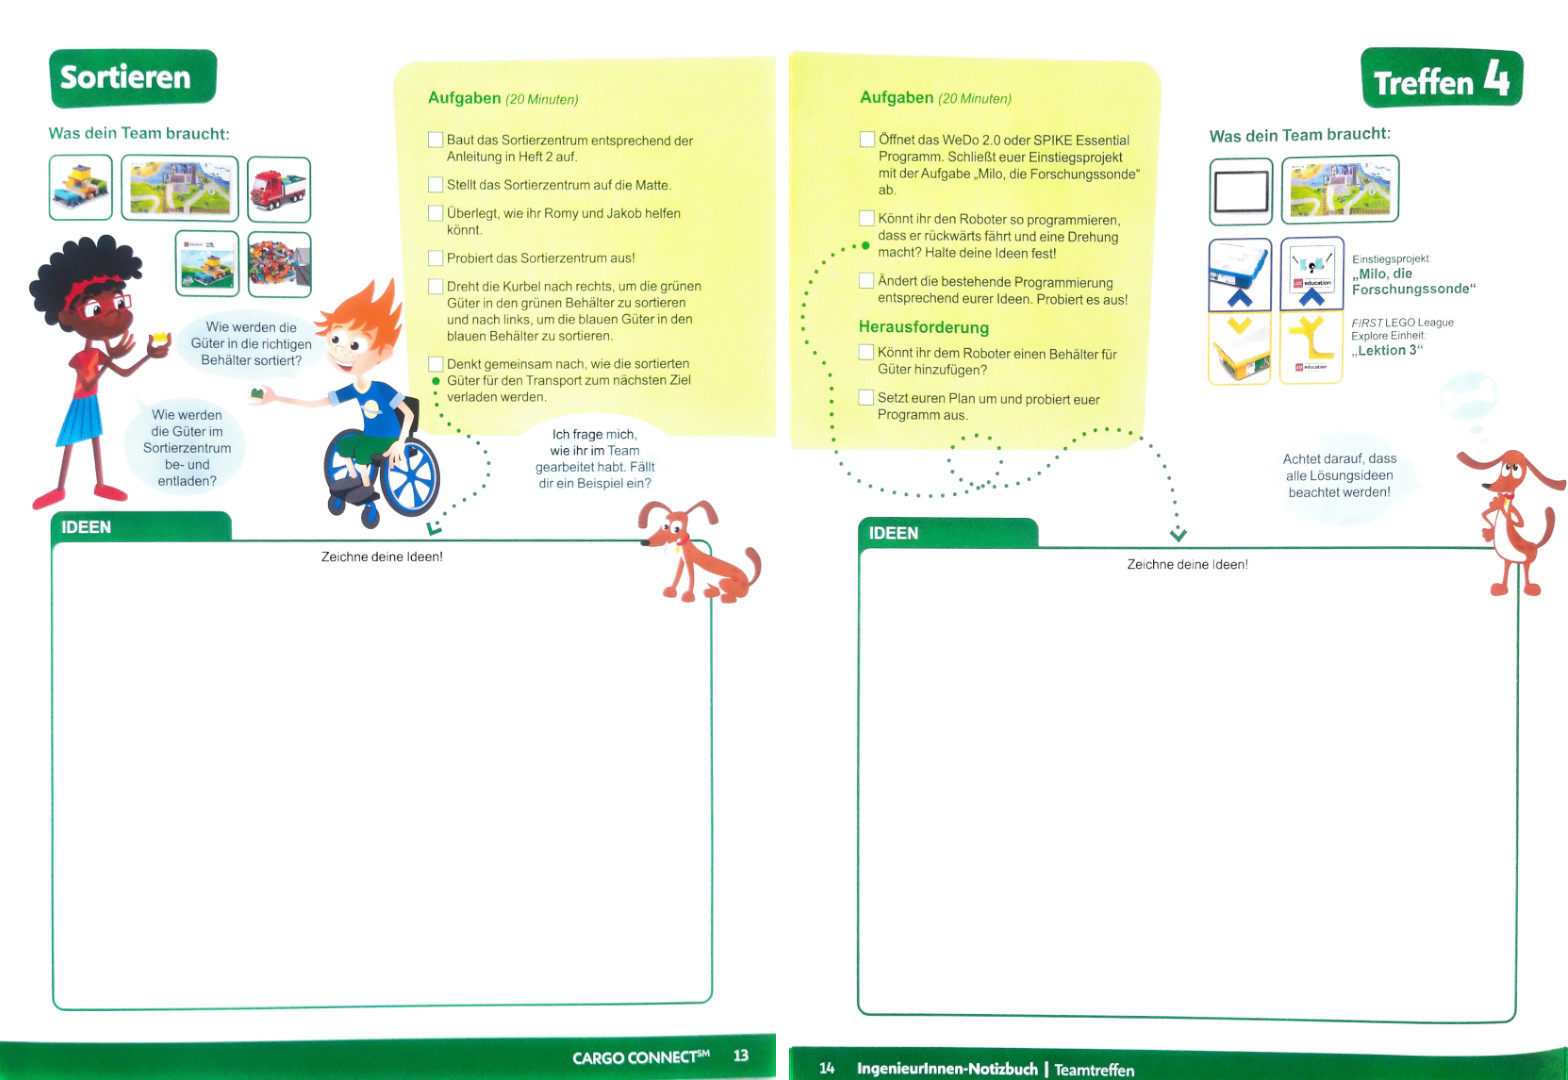
\includegraphics[width=0.3\textheight,angle=0]{img/Explorer}}
		\caption[Ausschnitt aus dem IngenierurInnen-Heft]{Ausschnitt aus dem IngenierurInnen-Heft}
		\label{img:explorer_heft}
	\end{figure}
	
\section{Ergebnisse des Computational Thinking Test}\label{sec:ErgebnisseCTT}
	\subsubsection{Vor Beginn des Workshops}
	\begin{table}[H]
		\centering
		\begin{tabular}{|
				>{\columncolor[HTML]{C0C0C0}}c |c|c|c|c|c|c|c|}
			\hline
			\textbf{Name} &
			\cellcolor[HTML]{C0C0C0}\textbf{Typ 1} &
			\cellcolor[HTML]{C0C0C0}\textbf{Typ 2} &
			\cellcolor[HTML]{C0C0C0}\textbf{Typ 3} &
			\cellcolor[HTML]{C0C0C0}\textbf{Typ 4} &
			\cellcolor[HTML]{C0C0C0}\textbf{Typ 5} &
			\cellcolor[HTML]{C0C0C0}\textbf{Typ 6} &
			\cellcolor[HTML]{C0C0C0}\textbf{Total} \\ \hline
			
		
			Henriette            & 6 & 5 & 7 & 2 & 2 & 3 & 25 \\ \hline
			Moritz               & 6 & 5 & 7 & 2 & 2 & 3 & 25 \\ \hline
			Heinz                & 6 & 5 & 7 & 2 & 1 & 3 & 24 \\ \hline
			Benny                & 6 & 5 & 7 & 2 & 0 & 3 & 23 \\ \hline
			Lulu                 & 6 & 4 & 6 & 2 & 2 & 3 & 23 \\ \hline	
			Mario                & 6 & 4 & 3 & 2 & 1 & 2 & 17 \\ \hline
			Sara                 & 6 & 2 & 7 & 0 & 1 & 1 & 17 \\ \hline		
			Jonas                & 0 & 2 & 3 & 1 & 1 & 3 & 10 \\ \hline
			\textbf{Maximalwert} & 6 & 5 & 7 & 2 & 2 & 3 & 25 \\ \hline
		\end{tabular}
		\caption{Erreichte Punkte pro Kategorie des BCTt}
		\label{tab:data}
	\end{table}
	
	In der obenstehenden Tabellen sind die Anzahl der Punkte aufgeführt, die die einzelnen Teilnehmer, hier mit Pseudonym aufgeführt, erreicht haben. Wie aus der letzten Zeile deutlich wird, sind unterschiedliche Maximalpunkte erreichbar. Daher wurden für die beiden folgenden Abbildungen die Werte dieser Tabelle auf 10 normalisiert. Dabei ist zu sehen, dass besonders in Kategorie 1, welche reine Sequenzen abfragte, und Kategorie 3, die den Umgang mit verschachtelten Schleifen prüfte, fast alle Probanden außer Jonas die volle Punktzahl erreicht haben, da er die Fragen nicht eindeutig beantwortet hatte und deshalb ihm keine Punkte gegeben werden konnte.	\\ 
	
	
	\begin{figure}[H]
		\centering
		\begin{tikzpicture}
			\tkzKiviatDiagram[scale=.5,label distance=.5cm,
			radial  = 5,
			gap     = 1,  
			lattice = 10]{Typ 1,Typ 2,Typ 3,Typ 4 ,Typ 5, Typ 6}
			%Jonathan
			\tkzKiviatLine[thick,color=blue,mark=none!20,opacity=1](10,8,4.285714286,10,5,6.666666667)
			%Annabell
			\tkzKiviatLine[thick,color=green,mark=none!20,opacity=.85](10,10,10,10,10,10)
			%Luise
			\tkzKiviatLine[thick,color=yellow,mark=none!20,opacity=.5](10,8,8.571428571,10,10,10)
			%Benny
			\tkzKiviatLine[thick,color=magenta,mark=none!20,opacity=.85](8.333333333,6,4.285714286,5,0,3.333333333)
			%Mohammed
			\tkzKiviatLine[thick,color=orange,mark=none!20,opacity=.85](10,10,10,10,5,10)
			%Yufei
			\tkzKiviatLine[thick,color=brown,mark=none!20,opacity=.85](10,4,10,0,5,3.333333333)
			%Henrik
			\tkzKiviatLine[thick,color=purple,mark=none!20,opacity=.85](0,4,4.285714286,5,5,10)
			%Namenslos
			\tkzKiviatLine[thick,color=teal,mark=none!20,opacity=.85](10,10,10,10,10,10)
			%Maximalwert
			%\tkzKiviatLine[thick,color=black,mark=none,
			%fill=black!20,opacity=1](10,10,10,10,10,10)
			\tkzKiviatGrad[prefix=,unity=1](1)  
			
		\end{tikzpicture}
		\caption[Auswertung]{Auswertung der Tests}
		\label{img:auswertung}
	\end{figure}
	
	Abbildung \ref{img:auswertung} verwendet die normalisierten Werte aus Tabelle \ref{tab:data}. Sichtbar wird hier besonders der Einbruch in der Kategorie für Bedingungen mit If und Else, nur ein Proband konnte hier alle Fragen richtig beantworten. Bei Kategorie 3 ist erkennbar, dass es hier wohl große Unterschiede zwischen den einzelnen Teilnehmern gibt, da hier die Extremwerte eine Differenz von etwas unter 6 Punkten, also fast 60\% Unterschied sichtbar wird. Auch die Typen 2 und 6 weisen ähnliche Muster auf, wobei bei Typ 6 die Differenz über 6 liegt. Typ 1 und Typ 4 dagegen ist bei allen Teilnehmern fast gleich gut, hier ist die Differenz der Extremen deutlich geringer.\\ 

	\begin{figure}[H]
		\centering
		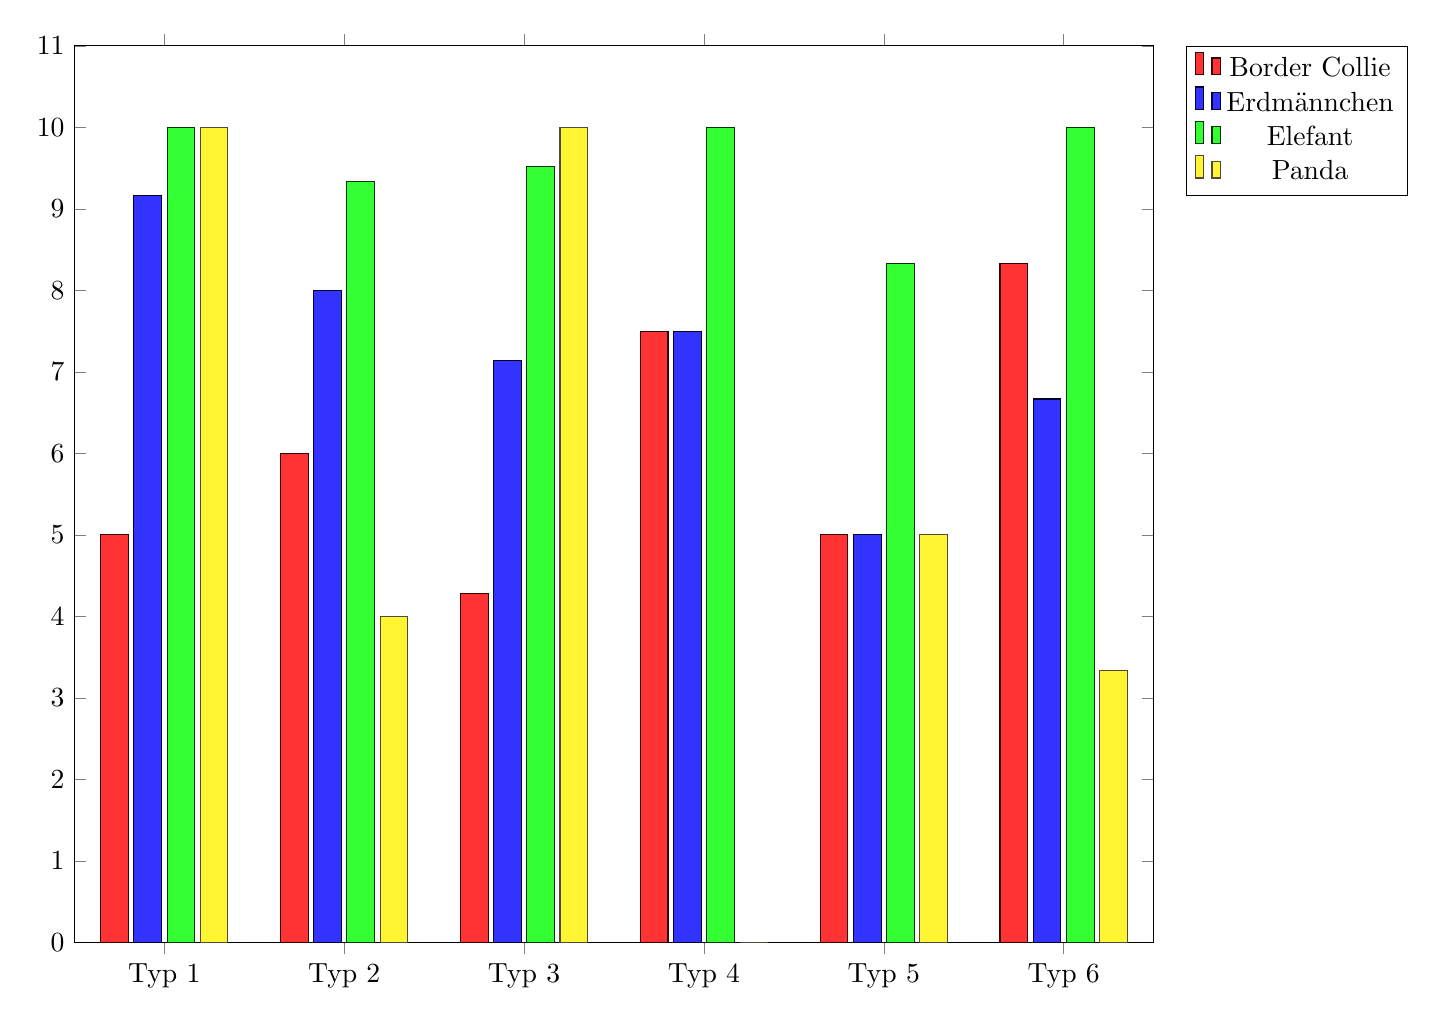
\begin{tikzpicture}
			\begin{axis}[
				ybar,ymin=0,
				symbolic x coords={Typ 1, Typ 2, Typ 3, Typ 4, Typ 5, Typ 6},xtick={Typ 1, Typ 2, Typ 3, Typ 4, Typ 5, Typ 6 
				}, scale = 2,legend pos=outer north east
				]
				%Border Collie
				\addplot[red!20!black,fill=red!80!white] coordinates
				{(Typ 1,5) (Typ 2,6) (Typ 3,4.285714286) (Typ 4,7.5) (Typ 5,5) (Typ 6,8.333333333)};
				%Erdmännchen 9,166666667	8	7,142857143	7,5	5	6,666666667
				\addplot[blue!20!black,fill=blue!80!white] coordinates
				{(Typ 1,9.16666667) (Typ 2,8) (Typ 3,7.142857143) (Typ 4,7.5) (Typ 5,5) (Typ 6,6.66666667)};
				%Elefant
				\addplot[green!20!black,fill=green!80!white] coordinates
				{(Typ 1,10) (Typ 2,9.333333333) (Typ 3,9.523809524) (Typ 4,10) (Typ 5,8.333333333) (Typ 6,10)};
				%Panda
				\addplot[yellow!20!black,fill=yellow!80!white] coordinates
				{(Typ 1,10) (Typ 2,4) (Typ 3,10) (Typ 4,0) (Typ 5,5) (Typ 6,3.33333333)};
				\addlegendentry{Border Collie}
				\addlegendentry{Erdmännchen}
				\addlegendentry{Elefant}
				\addlegendentry{Panda}
			\end{axis}
		\end{tikzpicture}
		\caption[Auswertung Durchschnitt]{Durchschn. Punkte pro Kategorie der einzelnen Typen, normalisiert}
		\label{img:auswertung_typus}
	\end{figure}

	Ebenfalls die normalisierten Werte verwendet auch Abbildung \ref{img:auswertung_typus}. Hierbei wird der Durchschnitt der einzelnen Typen pro Kategorie des Tests dargestellt. Auffallend ist besonders der Typ Border Collie und Elefant. Border Collie hat eine relativ geringe Durchschnittspunktzahl in den Testkategorien erreicht, Elefant dagegen erreichte in der Hälfte aller Kategorien den Maximalwert, in der anderen Hälfte kam dieser Typ nahe ans Maximum. Der Panda dagegen hat eine relativ hohe Streuung, die Werte liegen im kompletten Bereich von 0 bis inklusive 10.\\
	\subsubsection{Am Ende des Workshops}
	Aufgrund der Ergebnisse des \acrshort{bctt} mussten die Kinder am Ende einen schwereren Test bearbeiten, um eine bessere Aussage darüber treffen zu können, ob sie nun die Fähigkeiten des Computational Thinkings verbessern konnten.\\
	Aufgrund eines vorzeitigen Ausstiegs aus der Studie nahm Heinz nicht mehr am \acrshort{cctt} teil.
	\begin{table}[H]
		\centering
		\begin{tabular}{|
				>{\columncolor[HTML]{C0C0C0}}l |l|l|l|l|l|l|l|l|}
			\hline
			&
			\cellcolor[HTML]{C0C0C0}1 &
			\cellcolor[HTML]{C0C0C0}2 &
			\cellcolor[HTML]{C0C0C0}3 &
			\cellcolor[HTML]{C0C0C0}4 &
			\cellcolor[HTML]{C0C0C0}5 &
			\cellcolor[HTML]{C0C0C0}6 &
			\cellcolor[HTML]{C0C0C0}7 &
			\cellcolor[HTML]{C0C0C0}Total \\ \hline
			Henriette & 1 & 1 & 0 & 0 & 2 & 0 & 0 & 4  \\ \hline
			Moritz    & 4 & 3 & 3 & 2 & 4 & 0 & 0 & 16 \\ \hline
			Heinz     & - & - & - & - & - & - & - & -  \\ \hline
			Benny     & 3 & 2 & 3 & 1 & 2 & 0 & 0 & 11 \\ \hline
			Lulu      & 4 & 1 & 0 & 0 & 0 & 1 & 0 & 6  \\ \hline
			Mario     & 0 & 1 & 0 & 0 & 1 & 1 & 0 & 3  \\ \hline
			Sara      & 2 & 0 & 0 & 0 & 2 & 1 & 1 & 6  \\ \hline
			Jonas     & 1 & 1 & 1 & 0 & 0 & 0 & 0 & 3  \\ \hline
		\end{tabular}
		\caption{Erreichte Punkte pro Kategorie des CCTt}
		\label{tab:auswertungCCTT_kids}
	\end{table}
	Tabelle \ref{tab:auswertungCCTT_kids} zeigt das Abschneiden der Kinder in den jeweiligen Kategorien. Moritz und Benny stechen durch ihre hohen Punktzahlen deutlich hervor, ihnen gelang es in vielen Kategorien Punkte zu sammeln. Die restlichen Kinder dagegen taten sich eher schwer, viele Aufgaben korrekt zu beantworten, so dass diese nicht über ein Drittel der Punkte heraus kamen.



\pgfplotstableread[row sep=\\,col sep=&]{
	Typ &Border Collie&Erdmannchen&Elefant&Panda\\
	Typ 1     & 1.25  & 5 &10 &5 \\
	Typ 2     & 3.33 & 5 &6.67 &0 \\
	Typ 3    & 1.67 & 5 &5 &0\\
	Typ 4   & 0 & 2.5 &5 &0\\
	Typ 5   & 1.25  & 4 &5 &5\\
	Typ 6      & 2.5 & 0 &2.5  &5\\
	Typ 7 &0 & 0 &0 &3.33\\
}\dataCCTT

\begin{figure}[H]
	\begin{tikzpicture}
		\begin{axis}[ ybar,
			bar width=.3cm,
			width=\textwidth,
			height=.5\textwidth,
			legend style={at={(0.5,1)},
				anchor=north,legend columns=-1},
			symbolic x coords={Typ 1, Typ 2, Typ 3, Typ 4, Typ 5, Typ 6, Typ 7},
			xtick=data,ymin=0,ymax=11,
			ylabel={Anzahl erreichter Punkte}, xlabel = {Typ}]
			\addplot[red!20!black,fill=red!80!white] table[x=Typ,y=Border Collie]{\dataCCTT};
			\addplot[blue!20!black,fill=blue!80!white] table[x=Typ,y=Erdmannchen]{\dataCCTT};
			\addplot[green!20!black,fill=green!80!white] table[x=Typ,y=Elefant]{\dataCCTT};
			\addplot[yellow!20!black,fill=yellow!80!white] table[x=Typ,y=Panda]{\dataCCTT};
			\addlegendentry{Border Collie}
			\addlegendentry{Erdmännchen}
			\addlegendentry{Elefant}
			\addlegendentry{Panda}
		\end{axis}
	\end{tikzpicture}
	\caption[Auswertung Durchschnitt]{Durchschn. Punkte pro Kategorie der einzelnen Typen, normalisiert}
	\label{img:auswertung_typus_ctt}
\end{figure}




	In Abbildung \ref{img:auswertung_typus_ctt} zeigt sich, dass besonders die Elefanten und die Erdmännchen im Test deutlich besser abgeschnitten haben als die Kinder der anderen Persönlichkeitstypen. Interessant ist auch das Abschneiden des Pandas. Der Panda erzielte im \acrshort{bctt} eher weniger Punkte, ist aber der einzige Persönlichkeitstyp, welcher in den hinteren Kategorien gut abgeschnitten hat.

	\begin{table}[H]
		\centering
		\begin{tabular}{|
				>{\columncolor[HTML]{C0C0C0}}l |l|l|l|}
			\hline
			Name & \cellcolor[HTML]{C0C0C0}Test& \cellcolor[HTML]{C0C0C0}Computer & \cellcolor[HTML]{C0C0C0}erreichte Punkte \\ \hline
			Henriette & 20\%  & 20\%  & 19\%  \\ \hline
			Moritz    & 80\%  & 90\%  & 76.2\% \\ \hline
			Heinz     & -  & -  & -  \\ \hline
			Benny     & 50\%  & 80\%  & 52.4\% \\ \hline
			Lulu      & 50\%  & 80\%  & 28.5\%  \\ \hline
			Mario     & -  & -  & -  \\ \hline
			Sara      & 100\% & 100\% & 28.5\%  \\ \hline
			Jonas     & 60\%  & 90\%  & 14.3\%  \\ \hline
		\end{tabular}
		\caption[Selbsteinschätzung der Kinder]{Selbsteinschätzung der Kinder in Prozent im Verhältnis zu erreichten Punktzahl in Prozent}
		\label{tab:selbsteinschatzung}
	\end{table}
	
	Der \acrshort{cctt} hatte am Ende des Tests zwei Skalen zwischen 0 und 10, so dass die Kinder ihr Abschneiden im Test und ihren Umgang mit Computern selber bewerten konnten. Tabelle \ref{tab:selbsteinschatzung} zeigt, dass die Selbsteinschätzung ihres Abschneidens im Test nur manchmal mit der erreichten Punktzahl korreliert. Häufiger dagegen schätzen die Kinder sich als besser ein als das Ergebnis ihres Tests. 



\section{Parallelveranstaltung an der German University of Cairo}
Gleichzeitig zu dieser Studie fand an der \acrlong{guc} eine Parallelveranstaltung statt, die sich mit einem ähnlichem Thema befasste. Hierzu wurden ebenso über mehrere Termine vier Kinder in ähnlichem Alter wie die Kinder in dieser Studie beobachtet. Bei dieser Parallelveranstaltung ging es jedoch nicht um die Teilnahme an einem Wettbewerb, sondern die Kinder beschäftigten sich mit computerrelvanten Themen wie zum Beispiel Smart Home. Die Beobachtungen der Kinder wurden anschließend mit den Autoren dieser Studie geteilt. Die Kinder aus Ägypten absolvierten jedoch weder den Persönlichkeitstest noch die Computational Thinking Tests, weshalb über Zusammenhänge von Persönlichkeit und Lernfähigkeit keine Aussage gemacht werden kann. Lediglich können kulturelle Vergleiche zwischen den beiden Studien gezogen werden.
